\section{Proposed Rules}
\subsection{`auto` for variables}
These rules discuss `auto` type assignment w.r.t. variables. 
\insertcode{"Scripts/code5.java"}{Example assignment for variables}
\subsubsection{`auto` for primitive data types}
If auto is used for variables then for primitive types we propose the following type assignments based on the range of the value to be assigned: 
\begin{table}[h]
\centering
\caption{Range for `type` assignment}
\begin{tabular}{|p{2cm}|p{5cm}|p{5cm}|}
\hline
\textbf{Primitive Type} & \textbf{Lower Range}  & \textbf{Upper Range}\\
\hline
%byte 			& 	-128 				& 127\\
%short 			&   -32,768				&	32,767\\
int 			& 	-2,147,483,648		&	2,147,483,647\\
long			&	(-9,223,372,036,854,775,808 \ ... \ -2,147,483,649)	& (2,147,483,648 \ ... \ 9,223,372,036,854,775,807)\\
float			& 	1.4E-45				& 3.4028235E+38\\
double  		&	439E-324			& 1.7976931348623157E+308\\
boolean 		& true	& false\\
\hline
\end{tabular}
\end{table}
However, as per the language specifications if `l` is appended in the numeral literal it is considered as a long literal by default. Similarly, if `f` is appended in the decimal literal it is considered as a float literal by default. 
\subsubsection{`auto` for user defined objects}
Suppose we have the following Class arrangement as shown in Figure 8.1.

\begin{figure}
\centering
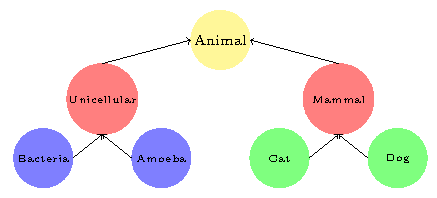
\includegraphics[width = 15cm]{diagram2.pdf}
\caption{Class Hierarchy Diagram\label{classhierarchy}}
\end{figure}

\insertcode{"Scripts/code6.java"}{Example assignment of user defined objects}

\subsection{`auto` for functions}
In the following code sample `x` would be assigned type `int` and `y` would be assigned type `Animal`. \\
\insertcode{"Scripts/code7.java"}{Basic function calling}

\subsubsection{Multiple return types for primitives}
\insertcode{"Scripts/code8.java"}{Multiple return types}
In case of conflicting return types of primitive data the function will return lowest common ancestor as shown in figure. Same rule will be followed for the wrapper class of these return types. 

\begin{figure}
\centering
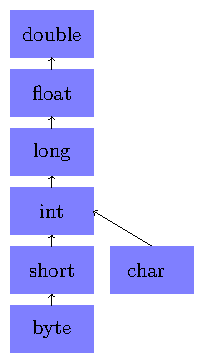
\includegraphics[width = 5cm]{diagram3.pdf}
\caption{Primitive data types coercision}
\end{figure}

\subsubsection{Multiple return types for classes}
\textbf{Parent $\leftrightarrow$ Child}\\
When the return type of a function is auto and it returns parent class as well as child class then after type resolution the parent class would be assigned as the return type of the function.

Based on the hierarchy of Figure 8.1 if we have the code as given in Listing 7 then the return type should be Animal.
\insertcode{"Scripts/code9.java"}{Multiple return types}
\textbf{Sibling $\leftrightarrow$ Sibling}\\
In case when the return type of the function is auto and it returns two sibling class in a class hierarchy then the return type of the function would be the lowest common ancestor in the inheritance hierarchy. 

Based on the hierarchy of Figure 8.1 if we have the code as given in Listing \ref{multireturntype1} then the return type should be Animal as it is the lowest common ancestor in the class hierarchy. 
\insertcode{"Scripts/code10.java"}{Multiple return types\label{multireturntype1}}
This is allowed because currently in Java the code given in Listing \ref{multireturntype2} is allowed. 
\insertcode{"Scripts/code11.java"}{Multiple return types\label{multireturntype2}}

\subsection{C/C++ Compiler}
In C++11 standards value assignment to `auto` variables cannot be deferred and the variable definition should be accompanied together with variable declaration.
Code given in Listing \ref{declareanddefine} is allowed but code given in Listing \ref{declareonly} gives error. 
\insertcode{"Scripts/code12.c"}{Immediate variable definition \label{declareanddefine}}
\insertcode{"Scripts/code13.c"}{Deferred variable definition \label{declareonly}}
C/C++ compilers are single parse compilers. Therefore, we need to give the function definition/declaration before actual function use. 
\subsubsection{Recursion}
The code given in Listing \ref{recurtionnotallowed1} and Listing \ref{recursionnotallowed2} should give error while the code given in Listing \ref{recursionallowed} is allowed. The reason is that we should know be able to deduce the  return type of functions in the first parse as C/C++ compilers are single parse.
\insertcode{"Scripts/code14.java"}{Not allowed\label{recurtionnotallowed1}}
\insertcode{"Scripts/code15.java"}{Not allowed\label{recursionnotallowed2}}
\insertcode{"Scripts/code16.java"}{Recursion allowed\label{recursionallowed}}

\subsection{Java Compiler}
We can allow the code given in Listing 15 in Java as Java compilers make multiple parse over the code. This is also the reason that in Java we can defer the function definition after function use because we can parse the code again to type check with the function definition. 
\insertcode{"Scripts/code17.java"}{Deferred variable definition}
In fact, in Java we can allow the use of `auto` keyword for function return type for cyclic dependencies as shown in Listing \ref{cyclicdependency1}. In Listing \ref{cyclicdependency1} the return type of all the functions will become `int`.
\insertcode{"Scripts/code18.java"}{Cyclic Dependency\label{cyclicdependency1}}
There is only one condition that it is actually possible to deduce the return type and there is not clash in return types. For instance the code given in Listing \ref{code:cyclicdependency2} will give compile time error as there is unresolved cyclic dependency of return types.
\insertcode{"Scripts/code19.java"}{Type deduction not possible\label{code:cyclicdependency2}}

However, the code given in Listing \ref{cyclicdependency3} is allowed and we can deduce the return type. 
\insertcode{"Scripts/code20.java"}{Cyclic dependencies\label{cyclicdependency3}}

\begin{figure}
\centering
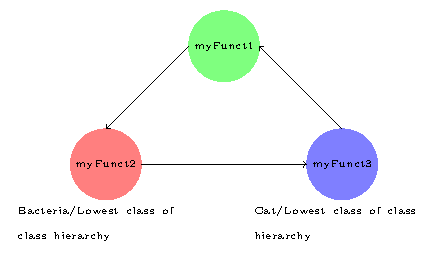
\includegraphics[width = 15cm]{diagram4.pdf}
\caption{Analysis of Listing 18}
\end{figure}